% !TEX root = ../HPCA2016.tex
\section{Architecture}
\label{sec:Architecture}

Our clustered migration mechanism was carefully designed to address key challenges associated with the migration problem. In this section, we present a complete description of our micro-architectural design, followed by a breakdown of all important design decisions made, along with the corresponding challenge addressed by each one.

\begin{table*}[t]
\begin{tabularx}{\textwidth}{ |X|X|X|X|X| }
  \hline
    \textbf{Challenge} & \textbf{Tradeoff} & \textbf{THM} & \textbf{HMA} & \textbf{MemPod} \\ \hline       
    Page Relocation & Flexibility Vs Time & Only 1 candidate \newline (Minimum / Very low)& No restrictions \newline (Max / High) & Intra-Pod migration \newline (High / Medium) \\ \hline
    Remap Table Size & Flexibility Vs Area & 1 entry per fast page \newline \TODO {XXkB} \newline (Minimum / Medium) & No remap table \newline 0 Bytes \newline (Max / Min) & 1 entry per fast page \newline \TODO{XXkB} \newline (High / Medium) \\ \hline
    Activity Tracking & Accuracy Vs Area & 8 bits per fast page \newline \TODO{XXkB} \newline (Medium / Low) & 16-bits per page \newline \TODO{XXkB} \newline (Max / Max) & 16-bits per fast page \newline \TODO{XXkB} \newline (High / Medium)\\ \hline
    Migration Trigger & N/A & Threshold based & Interval based & Interval based\\ \hline
    Tracking Organization & Simplicity Vs Parallelization & Fully Centralized \newline Serialized requests \newline (High / Min) & Fully distributed \newline (High / Max) & Semi-distributed \newline Pods operate independently \newline (High / High)\\ \hline
    Migration Driver & Communication cost & CPU \newline High latency \newline (Max) & CPU (OS) \newline High latency \newline (Max) & Pod \newline Very low latency \newline (Low)\\ \hline
    Migration Cost & Time & HW cost + communication \newline (Medium) & HW + SW + cold TLBs \newline (Max) & HW cost \newline (Min)\\ \hline
\end{tabularx}
  \caption{Breakdown of state-of-the-art designs}
  \label{tab:comparison}
\end{table*}

\subsection{Clustered Migration Architecture}

 Figure \ref{fig:architecture_complete} presents an overview of MemPod. MemPod's design was kept modular to facilitate system integration. A number of memory pods are injected between the LLC and the system's MCs. Each pod clusters a number of MCs and restricts migration  within the pod. To the rest of the system, pods are seen as MCs. With MemPod's transparent design, each pod will now be receiving all the requests originally addressed to any of the pod's MCs. 

A pod's operation when a memory request arrives would be to monitor the request, update any necessary migration-related counters and forward the request to the intended recipient MC. The migration logic within a pod does not need to be invoked during a response from any MC and could potentially be bypassed, saving some cycles. An obvious drawback of clustering MCs into pods is the serialization of potentially parallel requests to different MCs and as such, any counting scheme used by the pod -- as well as the actual forwarding of the request -- have to be as efficient as possible. 

\begin{figure}[h]
  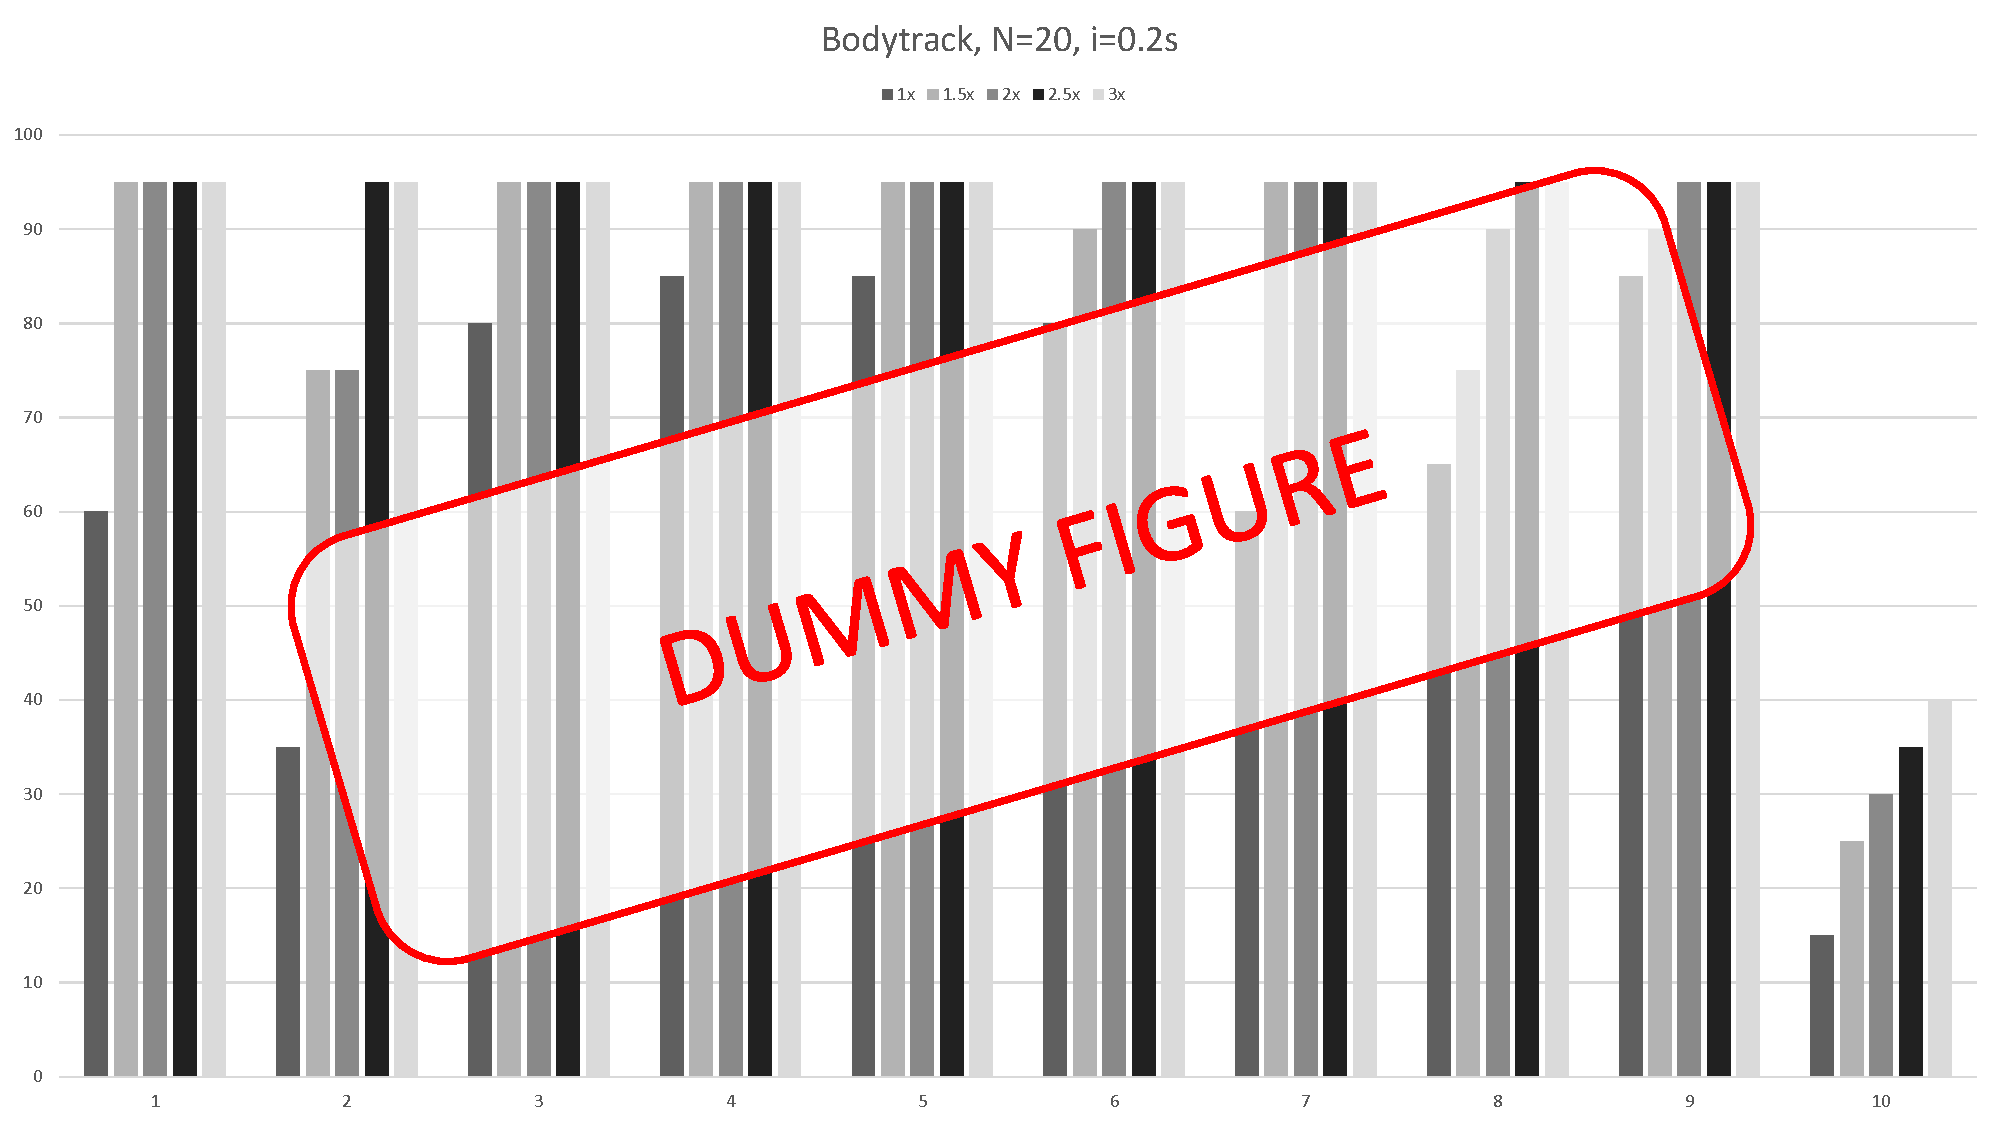
\includegraphics[width=0.46\textwidth]{figures/dummy.pdf}
  \caption{MemPod high-level architecture}
  \label{fig:architecture_complete}
\end{figure}

\begin{figure}[h]
  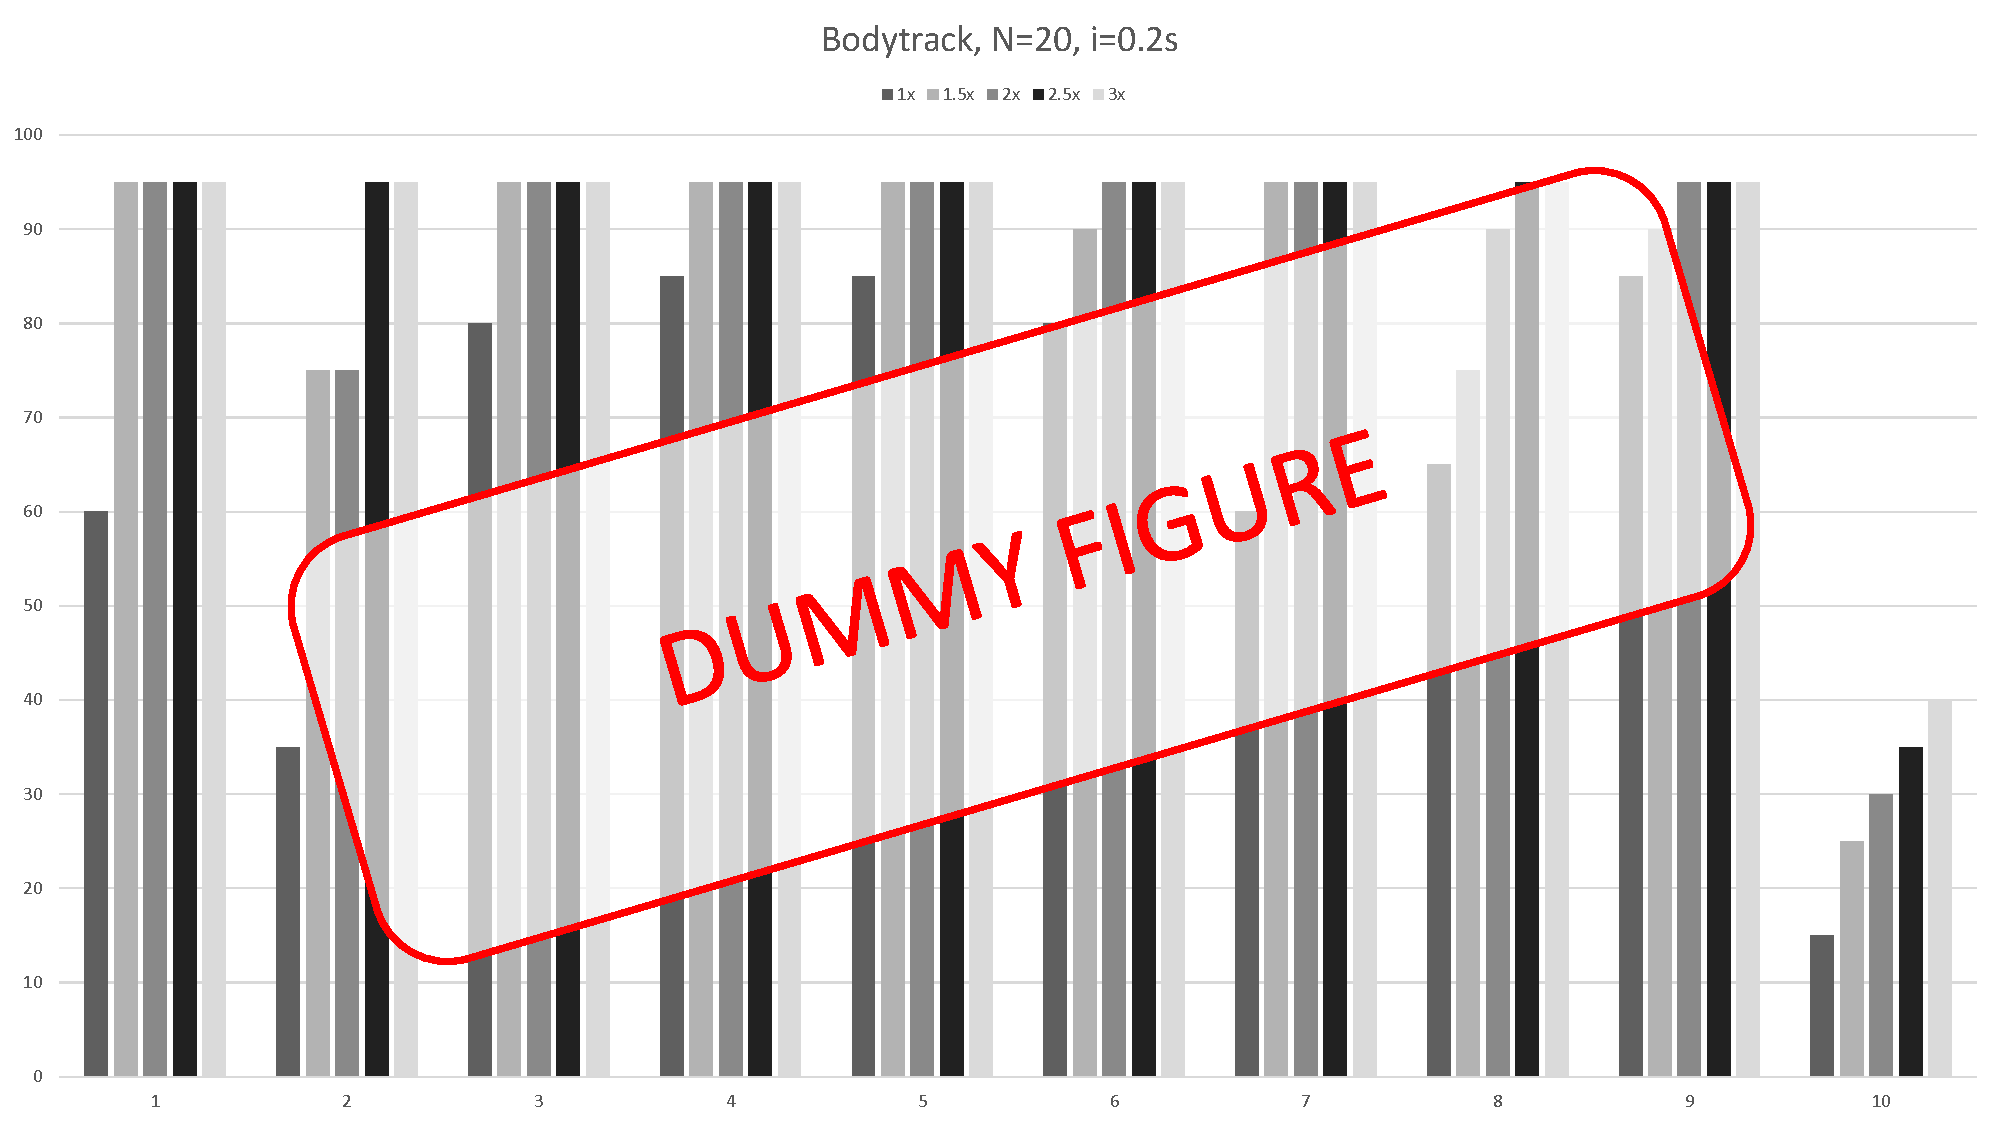
\includegraphics[width=0.46\textwidth]{figures/dummy.pdf}
  \caption{Major architectural Pod elements}
  \label{fig:architecture_pod}
\end{figure}

\subsubsection*{Memory Pod}
The major architectural elements of a Pod are presented in Figure \ref{fig:architecture_pod}. A Pod's remap structure includes the remap table as well as necessary decoding and hit detection logic. Counting logic is equally important for migration as the existence of a remap table and it's responsible for identifying the hot pages which will later be candidates for migration. Without reliable hot page detection, migration would be random and often counter-productive. Finally, migration logic is responsible for orchestrating a page swap between two MCs and updating the Pod's state.

During the design of a new system, the number of pods can vary arbitrarily given different constrains. A design with just one cluster would be equivalent to a centralized migration controller allowing any-to-any\footnote{Any-to-any Migration: Page migration without limits on source and destination. All MCs can migrate a page to any MC.} migration, while a design with a pod number equal to the number of MCs would imply that migration is disabled. The latter option would be completely redundant and is only used as an example. A reasonable number of Pods would be equal to the number of slow-memory MCs. In Figure \ref{fig:architecture_complete} we present a system with eight MCs for the fast, on-die stacked memory and four MCs for the slow off-chip memory. The use of four pods imposes few restrictions on migration possibilities, while forbiding migration between two slow-memory MCs. For the remainder of this paper, we set the number of pods to four.

The dollowing subsections provide detailed descriptions of all major elements of a migration management mechanism. We present MemPod's, THM's and HMA's approach to each element's design, as well as alternative designs. It's important to note that each of the following elements is independent from all the rest and future mechanisms could choose almost any element design combination in a plug-and-play fashion, with some exceptions. For example, the use of Majority Element Algorithm (MEA) activity tracking cannot work with threshold-based triggers.

\subsection{Page Relocation and Remap Table Size}
\label{sec:relocation}

Migration of memory pages can provide maximum benefits when no restrictions are imposed on the available migration locations. In other words, the optimal scenario for a migration policy would be the option of potentially filling the entire fast memory with migrated hot pages. On the other hand, more options require more bookkeeping and incur a higher cost. Flat address space memories do not have the luxury of a backing memory, like a 3D-stacked DRAM cache. Consequently, migrating a page implies swaping two pages to ensure the existence of exactly one copy for each of the participating pages. As such, migrating and swaping will be used interchangeably for the remainder of this paper.

A traditional remap table is a hash structure, indexed by a page's address and pointing to the migrated address if one exists. On a page migration, the remap table is updated to reflect the new address of a migrated pge. However, such a remap table is not enough when re-migration of pages is allowed. Figure \ref{fig:failed_remap} presents a scenario where a ''naive`` remap table fails. Figure \ref{fig:failed_remap}(i) shows the starting state of our memory before any migration, as well as the starting state of the remap table. For simplicity, we present the three memory locations needed by our example. Page 10 is assumed to be a fast memory page, while pages 100 and 200 are slow memory pages. The numbers inside the memory locations represent the content page's id. Figure \ref{fig:failed_remap}(ii) shows the state of memory and remap table after swaping pages 10 and 100. The content of page 10 is now page 100, and the content of page 100 is now 10. The remap table correctly states that requests to page 10 should be relayed to page 100 and vice versa.  Everything works as it should during this first migration, however Figure \ref{fig:failed_remap}(iii) shows the state after the second migration. Page 10 is now swaped with page 200. Such a migration would imply that page 100 (now held at 10) became cold and page 200 became hot. The contents are swaped and now page 10 holds page 200 and page 200 holds page 100. However, the state of the remap table is inconsistent. A request to page 10 would get forwarded to page 200, returning the wrong page.

The reason this remap table design fails is simply because pages are allowed to re-migrate -- like page 10 in our previous example -- while the remap table ''assumes`` the content held at a page address matches the page's ID.  There is only one solution to this problem: The migration logic needs to be aware of exactly where each page's contents are located at any given time. Such a requirement can be implemented in various ways:
\begin{description}
	\item[Safe and slow:] Always restore a forwarded page's contents before it participates in a new migration. For such an implementation, hot page count will have to be kept based on the content page instead of the real page Id. In the earlier example in Figure \ref{fig:failed_remap}, the second migration of page 10 implies that page 100 is cold, but in order to offer page restoration support, the second swapping of page 10 will have to imply that page 10 is cold. The cold page (10) will be restored back to address 10 from 100 and then moved to its new location. It's a minor modification that does not affect any other aspect of a migration mchanism.
	\item[THM approach:] Migration is restricted in segments. In a memory configuration with a 1:8 fast:slow memory ratio, exactly 9 pages compete for a position at the one fast memory page available. This solution is elegant enough to allow re-migration without extremely high storage overhead, limiting however the migration potential of memory pages. If two or more hot pages coexist in a segment, only one can reside in fast memory at any given time. At the same time, if none of the segment's pages are hot, the fast memory page slot cannot be utilized by some other segment's page.
	\item[HMA approach:] Any page can migrate to any other page address without the need of dedicated a remap table structure. The OS-based migration scheme imposes no limitations, since the OS takes care of updating the page tables and flush the TLB, however the cost of HMA's intervention and the penalties incurred from a cold TLB could sum up to very high values.
	\item[MemPod approach:] Migration is restricted within a Pod, but no intra-pod location restrictions are applied. A Pod's remap table is extended with a second field that holds the content page's id. During the second migration in our previous example, the issue was caused because we updated the remap entry of the holding page (10) instead of the entry of the content page (100). An attempt to recursively follow the remap table's entries until we figure out which one we should update risks looping infinitely because of cycles (For Example if page 10 is re-migrated back to address 10). Even if a smart algorithm is utilized to delete entries of non-migrated pages, the complexity of the recursive algorithm will only be bounded by the size of the remap table since in the worst case the entire table will be traversed. Figure \ref{fig:correct_remap} shows the memory and remap table states after the same page mirations as in Figure \ref{fig:failed_remap}. At the end of the second migration, the states of memory and remap table are consistent. It's important to note that a remap table entry is now points to a pair of values: (1) \textit{relay address} (i.e. where is the requested page located) and (2) \textit{content address} (Which page is currently held).
	\item[Alternative approach:] Recent works propose the use of arbitrarily small remap tables. When the remap table inevitably gets full two possible solutions exist: (a) Migration is disabled and (b) the OS is invoked to update page tables and flush the TLB. After OS's intervention, the remap table is cleared and migration remains active.
\end{description}

\TODO{Discuss the cost of MemPod and THM approach in terms of storage overhead. They should be similar.}

\begin{figure}[h]
  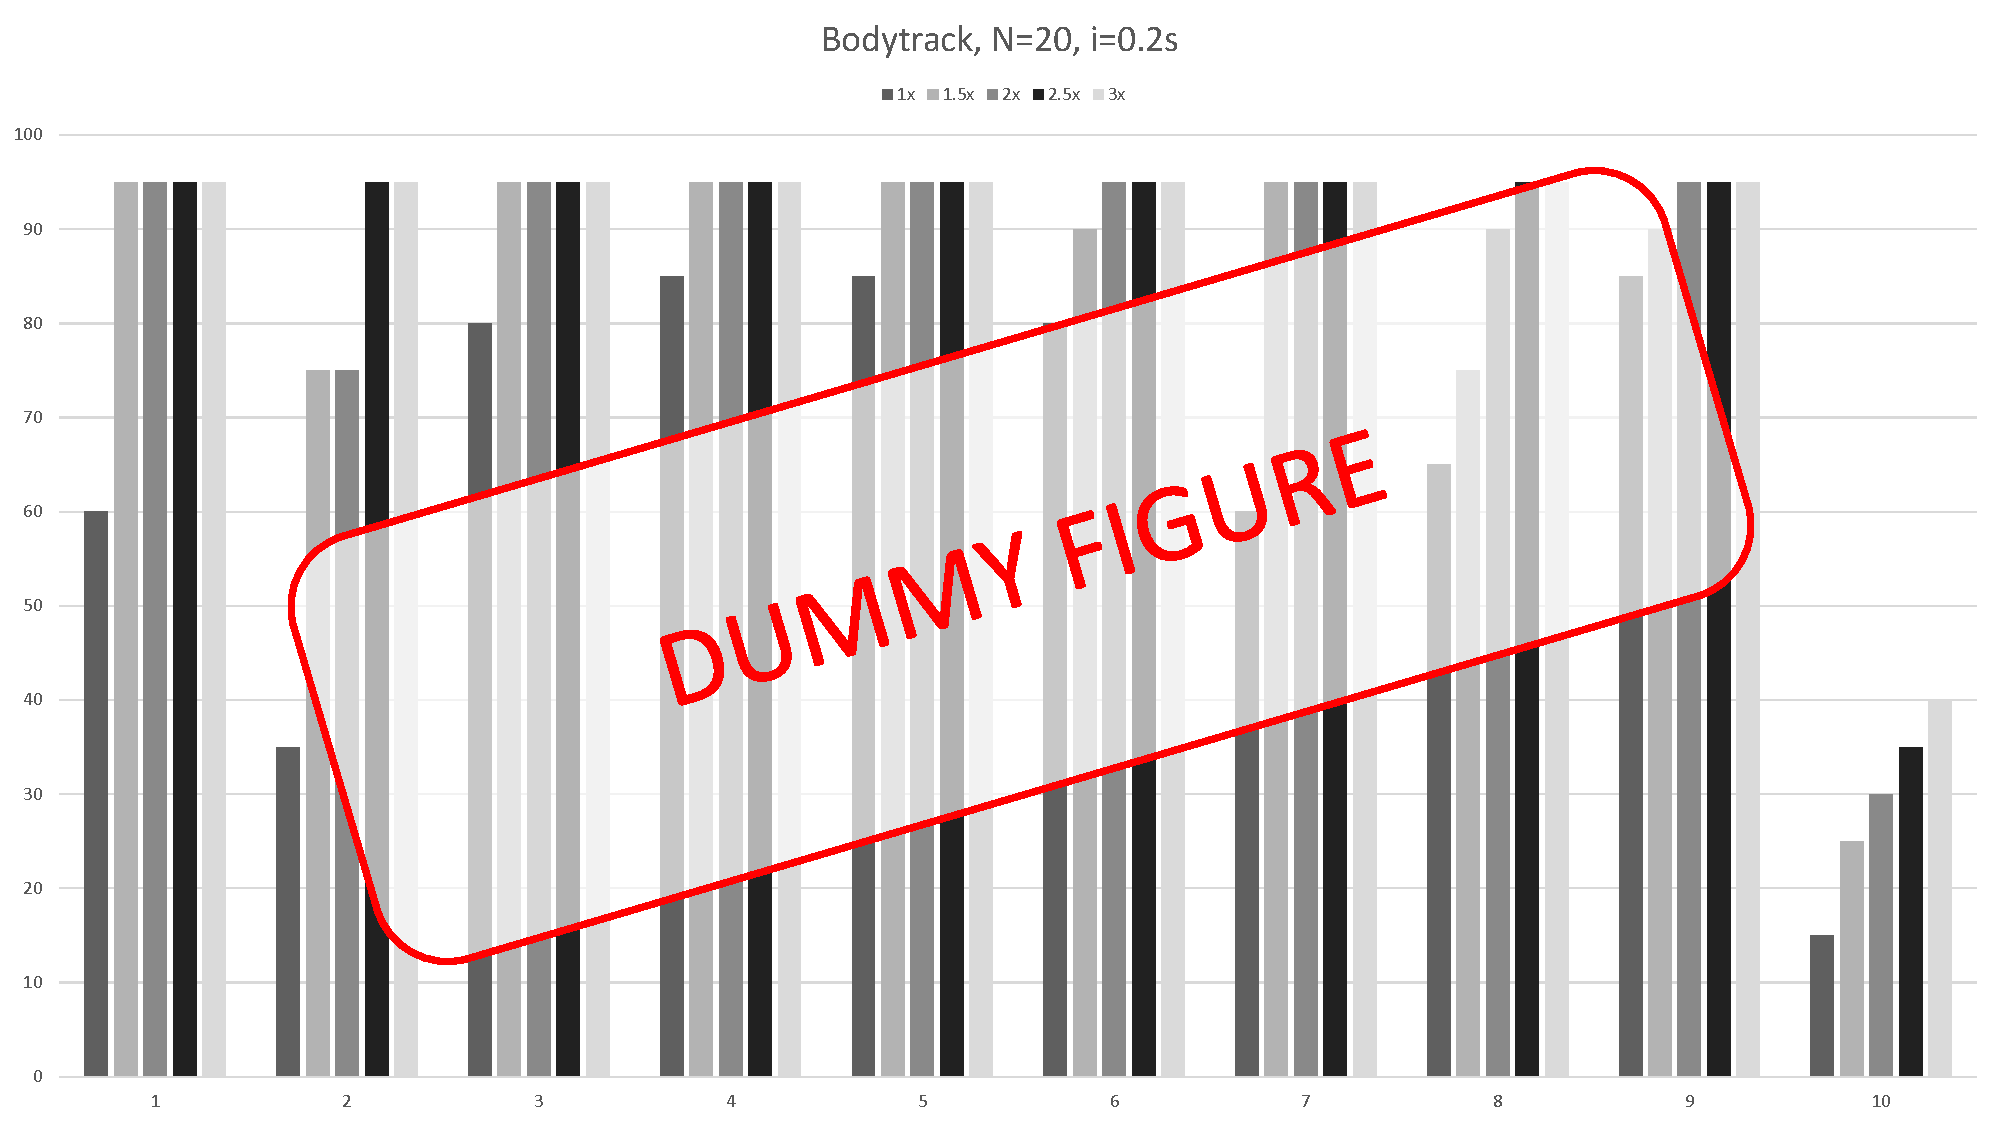
\includegraphics[width=0.46\textwidth]{figures/dummy.pdf}
  \caption{Naive remap table operation}
  \label{fig:failed_remap}
\end{figure}

\begin{figure}[h]
  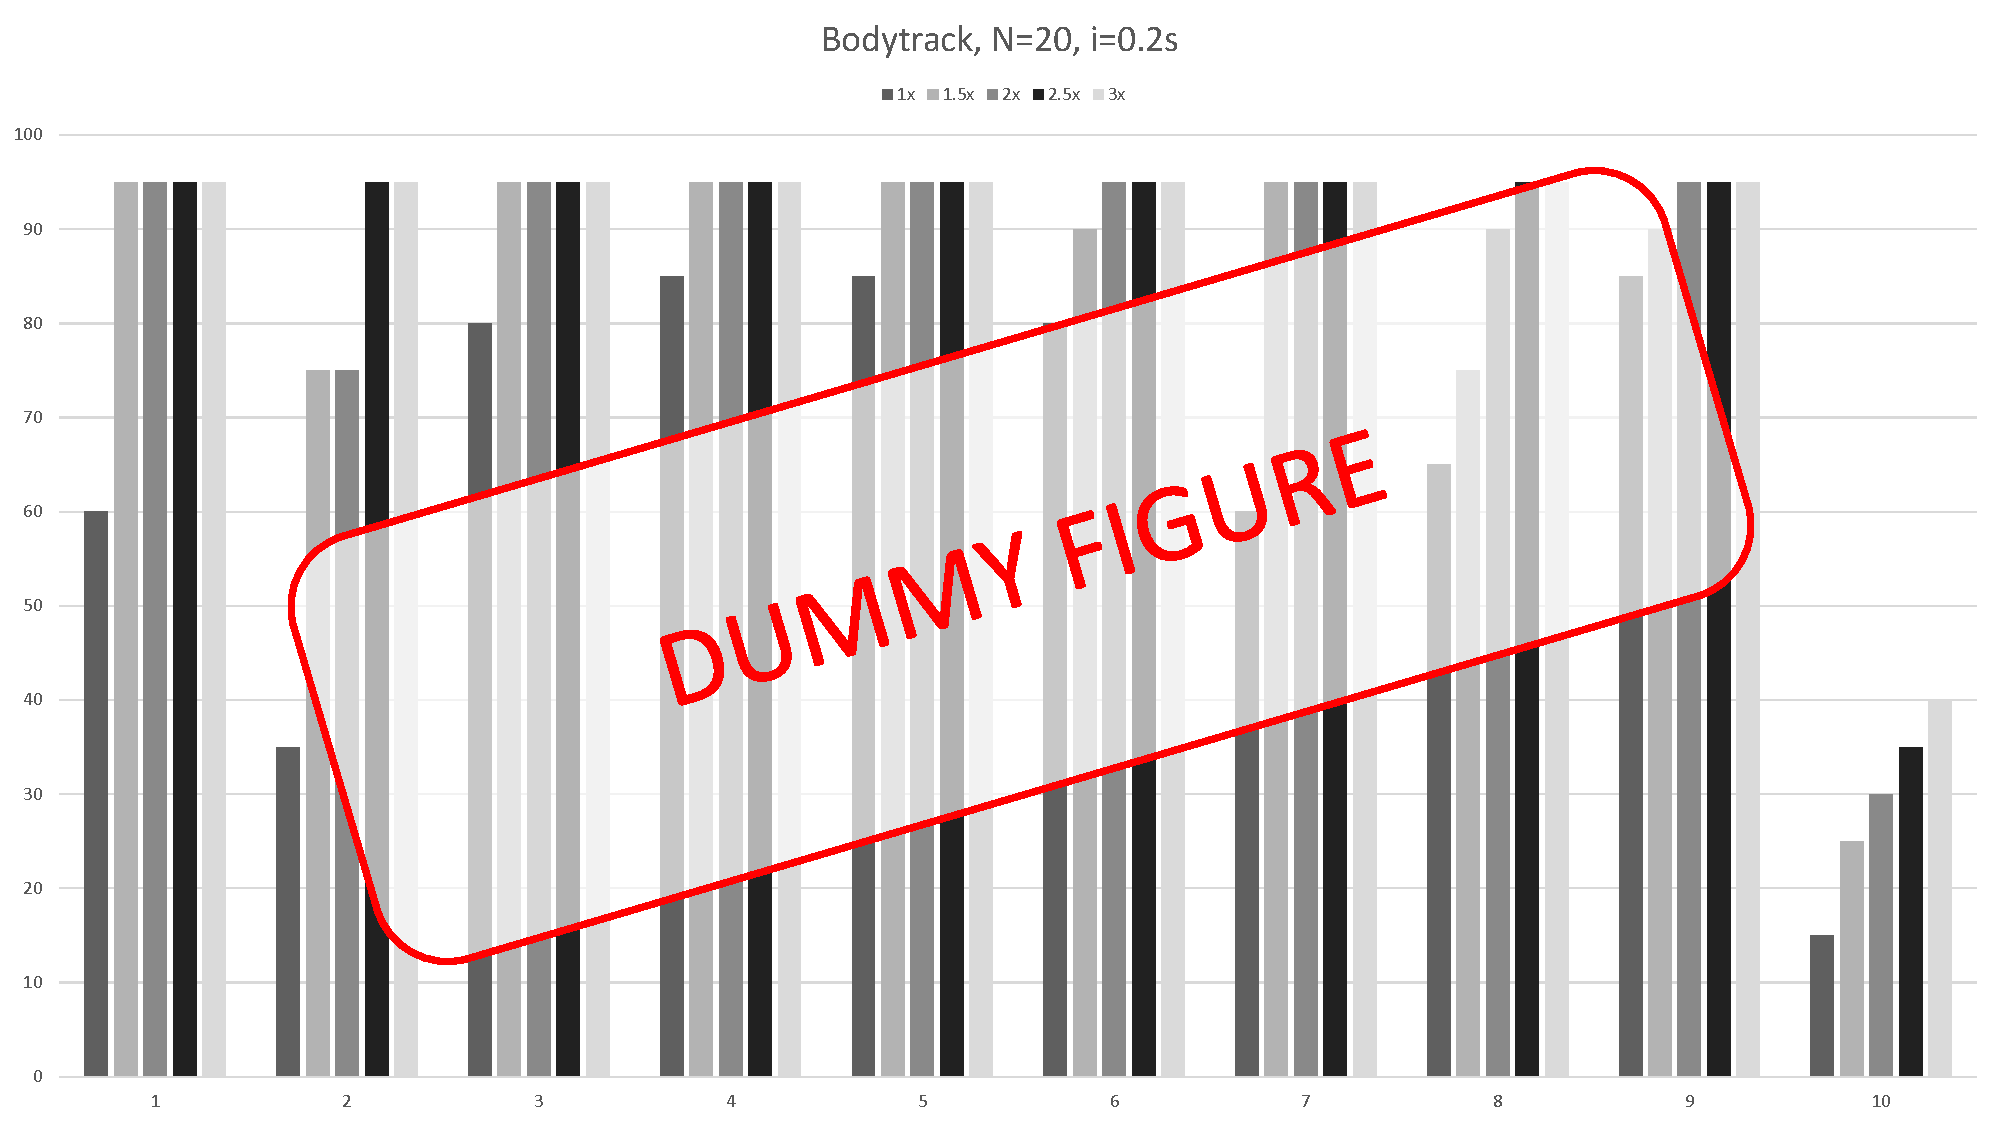
\includegraphics[width=0.46\textwidth]{figures/dummy.pdf}
  \caption{Remap design that allows re-migration}
  \label{fig:correct_remap}
\end{figure}


\subsection{Activity Tracking Mechanism}
\label{sec:tracking}

Activity tracking could be considered the most important element of any migration mechanism. In most migration studies, activity tracking becomes a synonym of identifying hot regions by counting the number of accesses. In a more generalilzed approach, it could potentially be extended to track patterns, parallelism, bit flips or any other information useful to the underlying mechanism. Along with the remap structure, activity tracking is the limiting factor in any migration policy. The overhead of maintaining a set of counters per migration segment, is often a bottleneck. 

MemPod utilizes an important observation to maintain a low activity tracking cost. Moving the hottest pages into fast memory is a commonly accepted approach, but not necessarily optimal. Several scenarios expose the failure of such an approach. For example, a page might become cold soon after it's migrated, wasting a space in fast memory. Another example arises when interval based migration policies are used. A cold page of the previous tracking cycle could become hot during the next interval. Strong indications exist that a combination of temporal as well as spatial locality has the potential of exposing better results. 

Frequently encountered solutions in the literature consist of increasing the activity tracking granularity (i.e. track a group of pages together), limiting the bits for each tracking counter, or simply paying the overhead for a complete tracking mechanism at the finer granularity. MemPod's activity tracking  is designed with a novel approach, using a Majority Element Algorithm (MEA) to track the hottest pages at a low cost. To the best of our knowledge, such an algorithm was never used in this context. THM also presents an interesting tracking approach, by utilizing competing counters for each segment.

Using counters for every memory segment supported by the migration mechanism obviously imposes extremely high area overhead but benefits in accuracy. Identifying the hottest pages however, also requires the often-overlooked sorting complexity. With the introduction of new memory technologies and the continuous capacity increase in memory capacities, it won't be long before even the most efficient sorting algorithm will require more time than we are willing to spend.

\begin{description}
	\item[THM approach:] One 8-bit competing counter tracks each memory segment. As described in Section \ref{sec:relocation}, THM restricts migration within segments. The competing counter is incremented by one when a page in slow memory is accessed and decremented by one when the segment's fast page is accessed. The counter's value is then monitored and can trigger migration. Competing counters represent a tradeoff between area overhead and accuracy. THM requires 8 bits per fast memory page making THM the most area-efficient as far as tracking is concerned. However, competing counters are susceptible to some error, since a cold page could potentially trigger migration and be placed in the fast memory.
	\item[HMA approach:] Full activity tracking per OS page (4KB) for all memory regions. THM uses the least efficient tracking mechanism in exchange for perfect knowledge at a fine granularity. Full activity tracking also introduces the complexity of sorting all the counters to identify hot pages. THM and MemPod do not require sorting.
	\item[MemPod approach:] MemPod requires one counter per hot memory page ranking close to THM's area efficiency. However, the set of MemPod's counters is capable of tracking pages \textit{from all memory regions.} using the Majority Element Algorithm presented in \TODO{cite}. For the remainder of this paper we will use the term ''MEA counters`` as a shorthand for MemPod's activity tracking. MEA is a simple, streaming algorithm which returns the (K) most frequently occuring elements in an array in linear time. As described in Section \ref{sec:related_work}, MEA is guaranteed to return the set of K hottest pages under certain assumptions that are not commonly held in a stream of memory requests. A sensitivity analysis of MemPod's tracking mchanism's accuracy is presented in the experimenal evaluation section. MEA strikes a balance between most frequently occuring and most recently used page addresses, a fortunate and welcomed consequence in locality exposure. As already discussed, asking for the K hottest pages does not necessarily mean that every other page is completely cold. For example, the K+1 page will usually be a good choice for migration as well. A new limitation arises when MEA counters are used: The system will be presented with the set of K hottest pages, however the counters' values cannot provide an order. The absolute hottest page could have a lower counter value than any other page.
\end{description}

Even with the most efficient tracking mechanism, future designs will soon be required to cache some of their counters while the rest are stored in memory to aleviate the area overhead. THM's segment-based counters are automatically cached along with their corresponding SRT entry and restored whenever necessary, at the cost of a memory access. It is also important to note that any counter update should be moved off the critcal path. Extreme accuracy is not necessary for correct operation. Even if the migration mechanism is not as accurate as it could be, all memory requests will be able to retrieve correct information as long as the state of memory and remap structure are consistent. Updating a remap table entry however, needs to be performed accurately without any ambiguity to aleviate the risk of inconsistent state.

\TODO{IDF:} With the recent growth in PIM (Processing-In-Memory, sometimes called Near-Memory Computation) mechanisms \TODO{[cite]}, future migration designs could rely on the PIM module to update the necessary counters, off the critical path and stored entirely in memory until it's time to use the actual counter values. The PIM approach \textit{eliminates} the need to store counters in SRAM circuits. Hypotheticaly, PIM could also be invoked for sorting the tracking counters.

\subsection{Migration triggers}
Deciding when to perform migration is as important as knowing which pages to migrate. Migration adds a significant delay to a system and as such it must be used wisely. Any penalties incurred whould be amortised by the performance improvement when placing a page in the fast memory. Requests that arrive while migration is performed have to be delayed to ensure functionaly correct behavior. Two very common triggers are used throughout the literature whenever state must be updated based on tracking information (such as MC scheduling, NUMA, DVFS etc.). Interval-based (or epoch-based) triggers occur with a steady frequency, while threshold-based solutions trigger without a predetermined frequency, whenever a threshold value is passed. 

Both interval-based and threshold-based approaches face the same challenge of identifying the optimal interval or threshold value. Identifying the appropriate value is not usually a trivial task. Factors like a system's architecture, application's behavior, as well as semi-random factors (for example DRAM will refresh more frequently under higher temperatures) make the optimal value differ from system to system. Designers usually opt for the value that provides the best results on average. The optimal value should not be too small since it will trigger some potentially expensive procedure frequently, but it cannot be too large since that usually leads to potential performance loses. 

As far as memory migration in flat address spaces is concerned, the state-of-the-art mechanisms trigger their migration procedures based on:
\begin{description}
	\item[THM approach:] THM uses a threshold-based mechanism. When the competing counter described in section \ref{sec:tracking} exceeds a threshold value, migration is triggered. THM will swap the page that triggered the event with the page currently residing in the segment's fast memory page. As a result, a small chance exists that a cold page was accessed at the right time to trigger migration and now it resides in fast memory. Such a mistake should be quickly get resolved however, since the cold page in fast memory should get remigrated soon enough. Each segment can trigger migration independently and asynchronously since no interval is used. THM risks very frequent migrations that will stall the stream of incoming requests until each swap is finished. \TODO{Check if they studied any of the previous two effects.} THM's authors identified the optimal threshold value as \TODO{XX}. 
	\item[HMA approach:] HMA uses an interval based mechanism. Upon each interval, HMA attempts to migrate as many pages in order to fill the fast memory. However with the high cost associated with the OS's intervention, management and the penalties of cold TLB force the interval value to be much larger. HMA authors identified the optimal timing interval to be as high as 1ms. \TODO{VERIFY}.
	\item[MemPod approach:] MemPod uses timing intervals. Like HMA, MemPod tried to fill the fast memory with hot pages on each interval. However, MemPod is transparent to the system and as such the need for costly OS intervention is waived. With the cost of a migration cycle kept to lower values, MemPod offers the possibility of a smaller interval time, which could potentially result in better performance. The optimal interval value is evaluated in the results section.
\end{description}

\subsection{Decentralization of migration logic}

The use of multiple MCs and multiple channels in today's memory organizations serves the purpose of exposing channel-level parallelism. Each channel can issue requests independently without any knowledge of other channels' states. Some migration mechanisms in the literature inherently ``assume'' a centralized migration controller in charge of monitoring traffic, while others attempt to implement a completely distributed mechanism. A centralized approach can be severely limiting. Current HBM memory technology allows up to 8 channels, while many processors are already designed with two or even more off-chip memory channels. Our evaluated system in this paper features a total of twelve memory channels. Channel number is predicted to increase in the near future \TODO{[cite]}. The channel parallelism capabilities will be entirely lost if we enforce request serialization due to migration-related activity tracking or remap table lookups. On the other hand, a fully distributed solution will eliminate all serialization, at the cost of all-to-all communication between each channel. An alternative to the communication cost would require OS intervention. MemPod's novel clustered architecture attempts to balance this tradeoff. 

As with most of the essential elements for migration presented in this Section, the system's designer can choose any level of centralization desired according to the specific design's constraints. As such, the body of work on migration covers the entire range:
\begin{description}
	\item[THM approach:] Even though not clearly stated in the THM proposal, it appears the authors opted for a centralized unit and consequently all channel parallelism potential is lost, placing THM last in our list in terms of parallelism potential. Decentralizing THM's migration controller appears to be possible due to the possibility of caching SRT entries, but in that case cache coherency becomes a concern. Race conditions could occur if the same SRT entry is simultaneously cached in different locations and its counter is modified. For this paper's evaluation section, we assume THM is fully centralized, as presented through figures in its proposal publication.
	\item[HMA approach:] HMA ranks at the top of our list, featuring a fully decentralized mechanism. It's important to note that HMA does not require a remap table and consequently one possible source of request serialization is automatically removed. Activity tracking is performed at each MC individually, where a controller will monitor the activity of its own pages. When HMA's migration is triggered, the OS collect all activity monitors from all the MCs before it proceeds with migration. Of course, collecting all this information from each MC by the OS consumes a considerable amount of cycles.
	\item[MemPod approach:] Clustering memory channels into Pods comes with significant benefits. First, assigning exactly one off-chip (slow) memory channel to each independent Pod ensures those channels can still issue requests in parallel. Being the slowest part of our memory hierarchy, keeping slow channels independent does not add delay to a potential bottleneck. Furthermore, each group of two on-chip (fast) channels can still operate in parallel. Some serialization is introduced between sibling fast channels, however with a Pod's light design and the high-bandwidth potential of those channels, the delay is amortized. Beyond channel parallelism, each Pod can hold all the migration-related structures, eliminating the need of retrieving information from each of its MCs at the beginning of a migration interval. \TODO{I'm trying to point out that a Pod keeps the structure size manageable because it handles less controllers. Other policies could hold all the information at a central point, but structures for 12 channels will be a log bigger thus slower. I think I'm not presenting my point correctly here.}
\end{description}

\subsection {Migration Datapath}
\TODO {Described later. Just remember to include it in the table.}

\subsection{Migration Cost}
Regardless of the choice for each migration element described so far, once migration is triggered, any migration manager has to follow the same steps: First, migration candidates need to be identified. Traditionally, one page (or a segment depending on the migration granularity) from the slow memory and one from fast memory. Both candidates need to be swapped. First they will be read and stored in temporary buffers and then written at their remapped locations. 

Describing the actual migration datapath is often overlooked in migration publications. Without dedicated page migration driver hardware, migration will have to be orchestrated by some CPUs. Consequences include communication delay, potentially some delay introduced at the processor's cache levels and the performance degradation caused by stalling those CPUs until migration is over. MemPod implements the migration driver within each Pod. Since the Pod has direct communication with the MCs, added delays are kept to a minimum. In HMA, the OS orchestrates everything. Some CPUs have to be stalled and used to service the OS interrupt, causing the migrated pages to traverse through communication mediums and caches on each way. THM does not describe the datapath in detail. We assume the CPUs are used in this case too.

We assume that channel parallelism is utilized when reading and writing the candidate pages. In other words, the two read commands will be sent in parallel, as well as the write commands that follow. Consequently, The hardware penalty for one page swap is the time required to read from and then write to the slow memory. We also assume that writing the two candidates back occurs a row buffer hit since the page was just opened in the previous step. When consequtive swaps happen, as in the case of HMA and MemPod, all swap reads are assumed to result in row buffer misses. In this study, we evaluate all mechanisms under the same memory organization and as such, the hardware swap penalty is the same regardless of the mechanism. However, each mechanism introduces some unique penalties:
\begin{description}
	\item[THM] does not introduce a cost for identifying the candidate pages since it follows a deterministic algorithm. The page that caused the competing counter to exceed the set threshold will be the slow memory candidate, while there is exactly one fast page candidate per segment. Furthermore, only one swap is executed at every triggered migration, setting te cost per migration equal to the hardware cost.
	\item[HMA ] attempts to fill the entire fast memory with migrated pages. The number of swaps that will be performed per interval can be as high as the number of pages in fast memory. Inevitably some hot pages will already reside in the fast memory. We modeled HMA to not attempt migration of those hot pages. Such an approach could compicate finding a fast-memory candidate page, although with HMA's full activity tracking counters, and since sorting is a necessary operation at every interval, this problem can be reduced to the simple task of following the sorted activity list backwards (i.e. It's easy to find the coldest fast-memory page). Unfortunately, HMA introduces costs that are hard to estimate. Traversing and updating page tables and flushing TLBs is part of the cost introduced by the OS. On top of that, the effect of a cold TLB can penalize severely all running applications.
	\item[In MemPod,] similar to HMA, each Pod tries to fill the entire fast memory assigned to it. With the use of MEA counters, identifying the fast-memory page candidate is as simple as checking that it's not part of the N hot pages. The identification algorithm starts at the very first fast memory location and iterates sequentially until it detects a page address that is not in the set of hottest pages. For the next migration, the identification algorithm simply continues from where it was left. If a hot page already resides in the fast memory it's ignored. Since we have exactly N MEA counters, we guarantee that the fast memory will have enough pages to accommodate all hot pages.
\end{description}

\TODO{Give numbers for hardware migration penalty}

\subsection{Scalability to Future Memory Capacities}
Assuming memory capacity in the order of tens of Terabytes, SRAM requirements for activity tracking and remap tables could become unfeasible. Caching part of the migration logic and using part of main memory as backing storage seems necessary. An analysis on the impact of such caching, as well as the optimal cache size is presented in the experimental evaluation section. MemPod's semi-distributed architecture allows caching without any action required to protect against race conditions because of the utilization of independent Pods that never share information.

At such capacity levels, centralized migration controllers will no longer be sustainable due to the severity of the introduced serialization penalty. Assuming the driving force behind memory capacity's tremendous scaling are future applications, it's safe to assume that memory traffic would also scale up, as well as sustainable bandwidth expectations. 

Alternative approaches described in this Section limit the size of the remap table at the cost of disabling migration when full, or invoking the OS before migration resumes. This approach could also be incorporated in future migration mechanisms. We should note that with a limited remap table size, or even an available number of counters less than the number of fast pages, MemPod would still be able to migrate \textit{any} slow memory page to the limited set of fast pages available for migration, in contrast to THM, where only those segments that happened to fit in the new limited size will be able to migrate, forbidding migration of the rest of the slow pages. HMA would remain intact from this limitation since no remap tables are necessary.

\subsection{Discussion and comparison}
\TODO{Talk about limits in the size of remap tables/counters just fr the sake of argument. How would each mechanism handle it?}



















































